\subsection{Class Diagram}
This section describes the various classes used to manage the two REST services ListFriendsRR and GamePlayerRR.
\subsubsection{ListFriendsRR}
\begin{figure}[htb] 
    \centering
    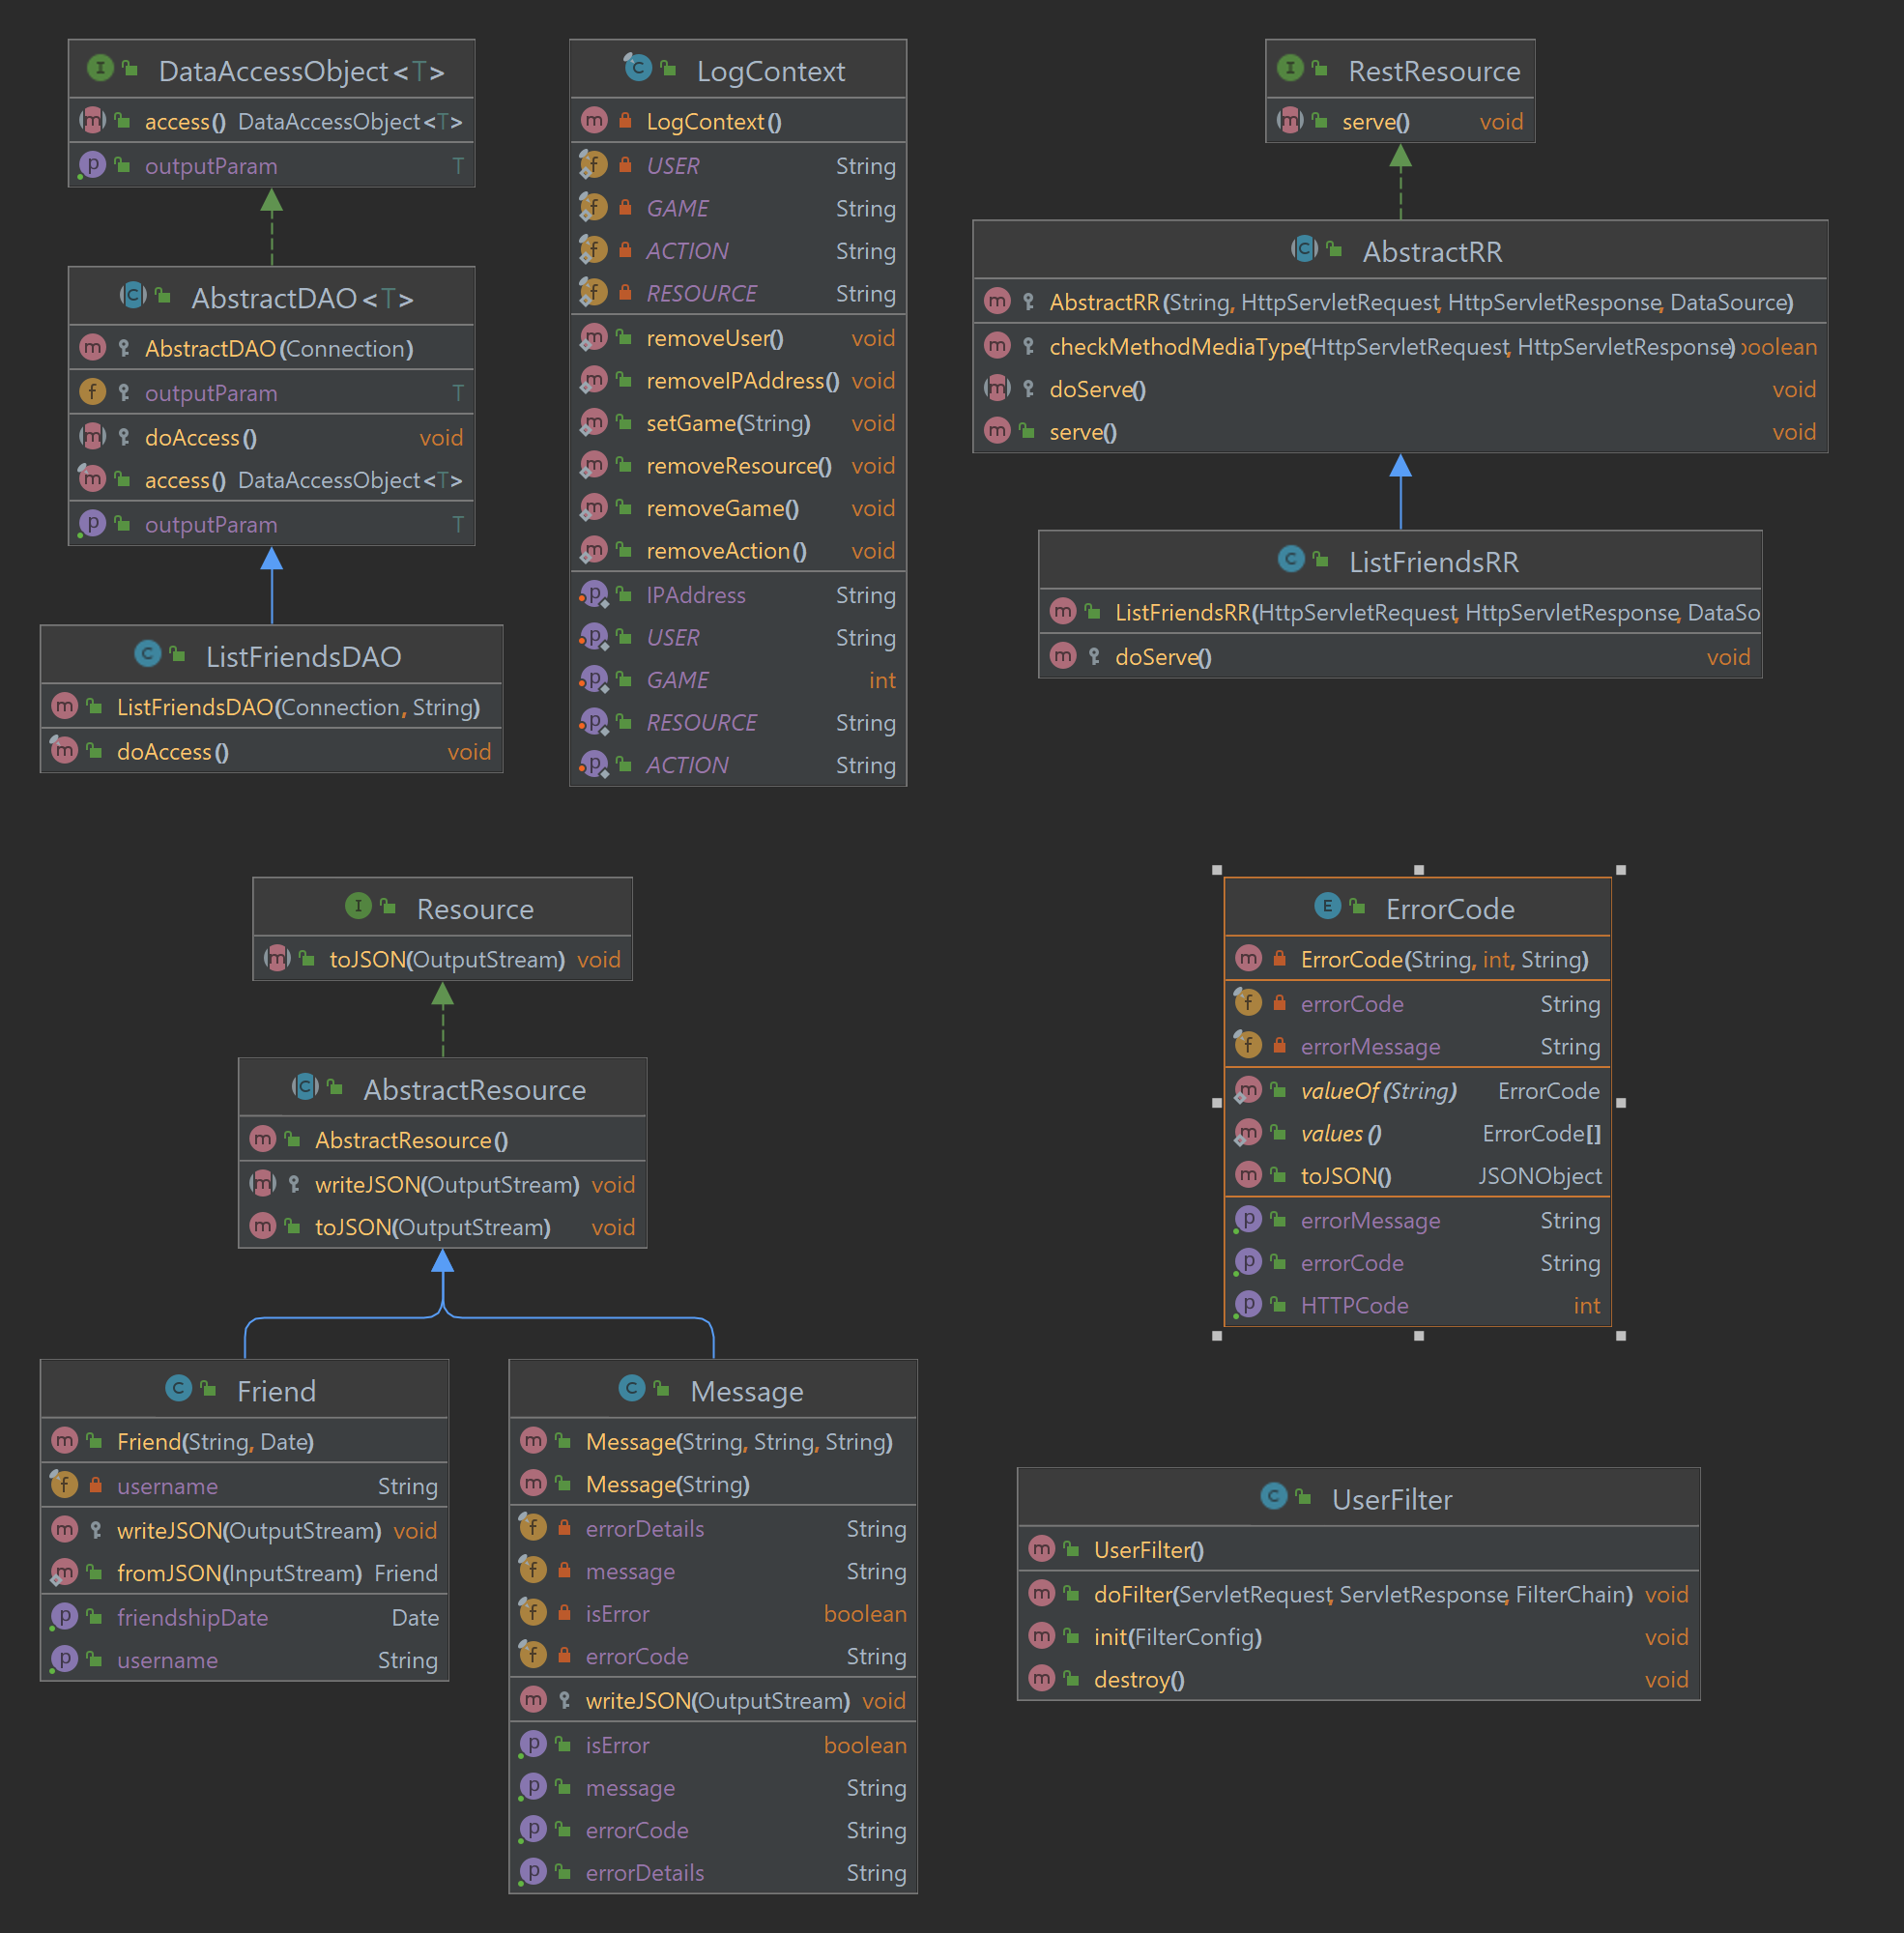
\includegraphics[height=9cm]{images/class_diagram/list_friend_diagram.png}
    \caption{List friend diagram}
    \label{fig:list_friend_diagram}
\end{figure}
%ListFriendsRR

The class ListFriendsRR extends the AbstractRR class, which represents the basic functions for every REST resource; ListFriendsRR implements the doServe() function, which is used to handle the request to view all the friends of a particular user.
%ListFriendsDAO
This REST resource communicates with the database and retrieves the list of all friends using the ListFriendsDAO class, which extends AbstractDAO; ListFriendsDAO implements the doAccess() function, which is used to access the database and execute the query to retrieve the list of all friends of the user.
%ErrorCode
This REST resource utilizes error codes implemented through the ErrorCode class, which implements functions like toJSON(), useful for converting errors into a JSON file, and valueOf(string s), useful for returning the value of a specific field passed as input.
%LogContext 
This REST resource utilizes LogContext to manage logs within the server, implementing various functions to set the values associated with logs (user, IP, game, action).
%friend 
This REST resource also utilizes "friend" to manage various instances of friends saved in the database, implementing toJSON() functions that create a JSON file representing an object, and fromJSON() functions that create a list of friends from a JSON file. These functions are inherited from the AbstractResource class, which represents the abstract resource.
%Message 
Additionally, this REST resource utilizes "Message" to manage all the various messages returned by the various REST resources, implementing toJSON() functions that create a JSON file representing an object. These functions are also inherited from the AbstractResource class.
%UserFilter
Finally, access to this REST resource is managed by the UserFilter filter, which implements filtering logic for user login and implements the doFilter() function to execute this check.


\subsubsection{GamePlayerRR}
\begin{figure}[htb] 
    \centering
    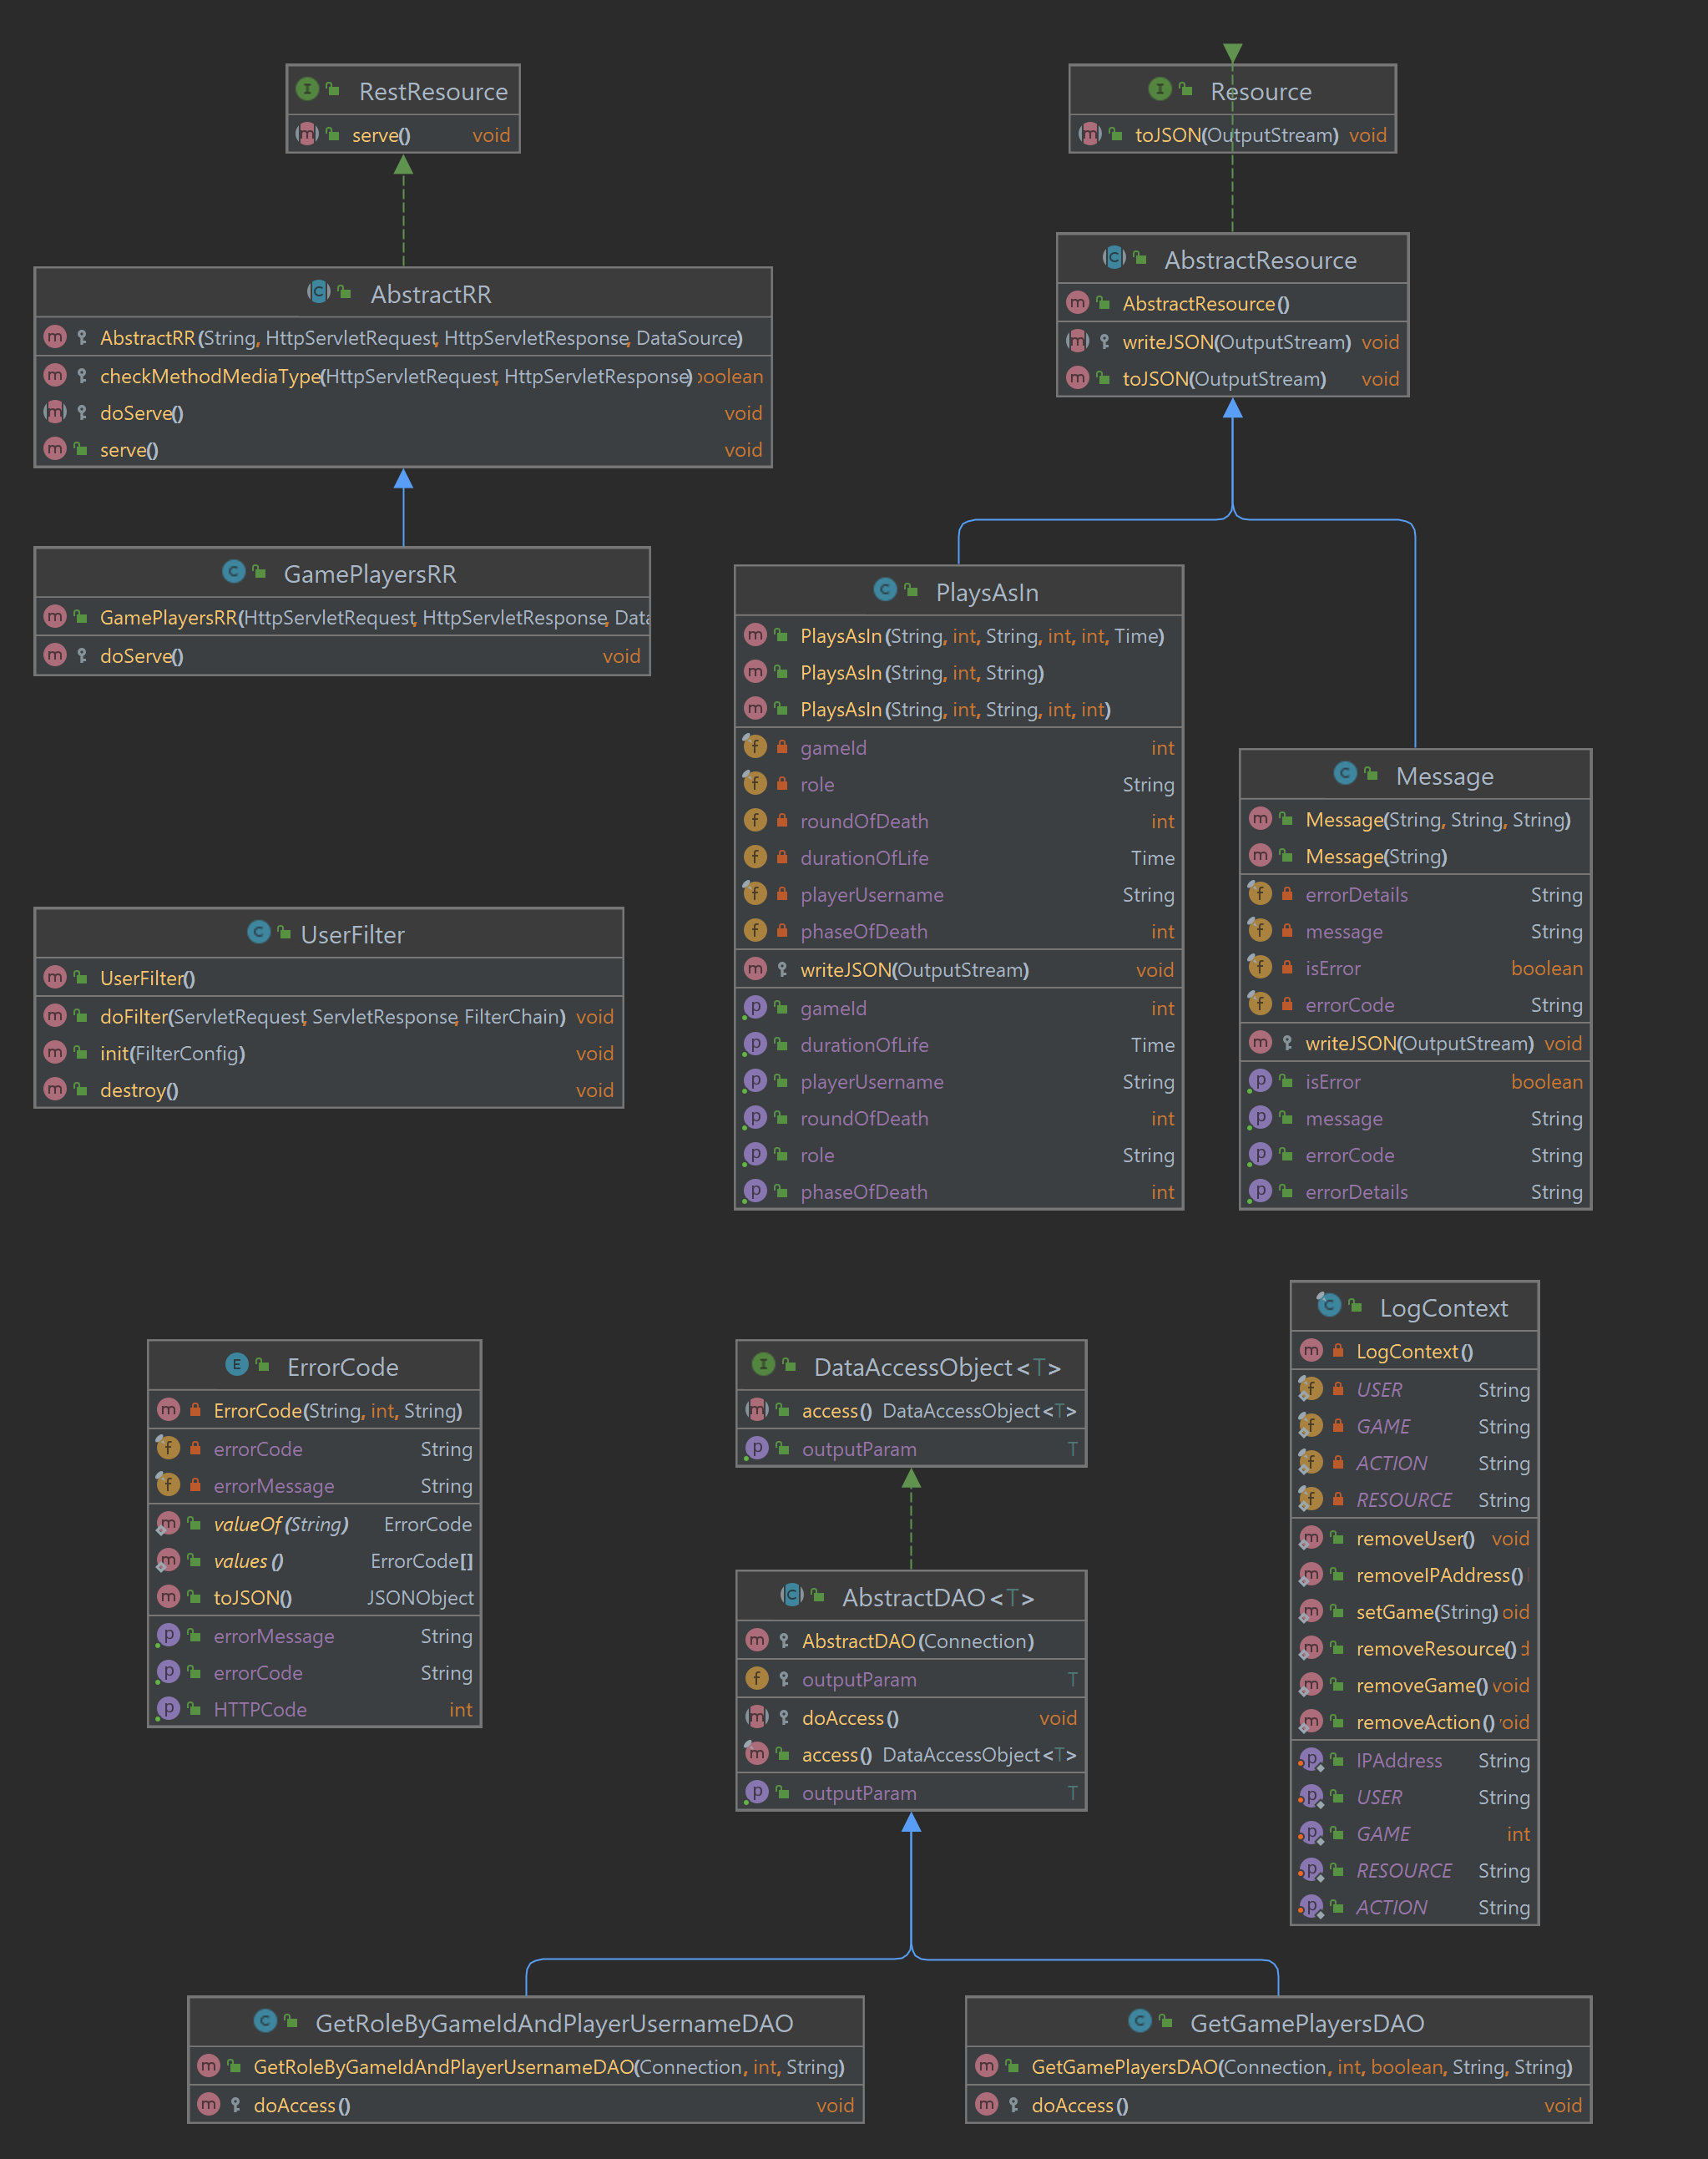
\includegraphics[height=10cm]{images/class_diagram/game_Player_diagram.png}
    \caption{List friend diagram}
    \label{fig:list_friend_diagram}
\end{figure}
%GamePlayerRR

The class GamePlayerRR extends the AbstractRR class, which represents the basic functions for every REST resource; GamePlayerRR implements the doServe() function, which is used to handle the request to get all player in game with a specific role.
%GetRoleByGameIdAndPlayerUsernameDAO
This REST resource communicates with the database and retrieves the list of all role associated with a user in a game using the GetRoleByGameIdAndPlayerUsernameDAO class, which extends AbstractDAO; GetRoleByGameIdAndPlayerUsernameDAO implements the doAccess() function, which is used to access the database and execute the query to retrieve the list of role
%GetGamePlayersDAO
This REST resource communicates with the database and retrieves the list of all player  in a game using the GetGamePlayersDAO class, which extends AbstractDAO; GetGamePlayersDAO implements the doAccess() function, which is used to access the database and execute the query to retrieve the list of all player in a game.
%PlayAsIn 
This REST resource also utilizes "PlayAsIn" to manage various instances of PlayAsIn saved in the database, implementing toJSON() functions that create a JSON file representing an object. These functions are inherited from the AbstractResource class, which represents the abstract resource.
%Message 
Additionally, this REST resource utilizes "Message" to manage all the various messages returned by the various REST resources, implementing toJSON() functions that create a JSON file representing an object. These functions are also inherited from the AbstractResource class.
%ErrorCode
This REST resource utilizes error codes implemented through the ErrorCode class, which implements functions like toJSON(), useful for converting errors into a JSON file, and valueOf(string s), useful for returning the value of a specific field passed as input.
%LogContext 
This REST resource utilizes LogContext to manage logs within the server, implementing various functions to set the values associated with logs (user, IP, game, action).
%UserFilter
Finally, access to this REST resource is managed by the UserFilter filter, which implements filtering logic for user login and implements the doFilter() function to execute this check.




